\documentclass[10pt,letterpaper]{article}

% to do (5/16)

%% put more sparkles around writing OED in a program. Why is this clever and useful?

%% introduce max Entropy prior early (could also be interpolation between max ent and the predictive)
%%%% results of sequence prediction (formerly, "randomness") w.r.t. maxEnt vs. predictive (discuss why we think maxEnt is giving a better prediction here)

%% Figure 3 histogram: vertical line with AIG
%% create n_subjects analysis figure (a la FIgure 3, line plot) for sequence prediction... bootstrap up to n=100 to observe crossover

% if you need to pass options to natbib, use, e.g.:
% \PassOptionsToPackage{numbers, compress}{natbib}
% before loading nips_2016
%
% to avoid loading the natbib package, add option nonatbib:
\usepackage{cogsci}
\usepackage{pslatex}
\usepackage[natbibapa]{apacite}

%\usepackage{nips_2016}

% to compile a camera-ready version, add the [final] option, e.g.:
% \usepackage[final]{nips_2016}

% \usepackage[utf8]{inputenc} % allow utf-8 input
% \usepackage[T1]{fontenc}    % use 8-bit T1 fonts
%\usepackage{hyperref}       % hyperlinks
\usepackage{url}            % simple URL typesetting
\usepackage{booktabs}       % professional-quality tables
\usepackage{amsfonts}       % blackboard math symbols
\usepackage{nicefrac}       % compact symbols for 1/2, etc.
% \usepackage{microtype}      % microtypography
\usepackage{amsmath}
\usepackage{mathtools}
\usepackage{fancyvrb}
\usepackage{multirow}
\usepackage{color}
\usepackage{textcomp}
\usepackage[scaled=0.8]{inconsolata}


% HT http://tex.stackexchange.com/a/151987/41154
\DeclarePairedDelimiterX{\infdivx}[2]{(}{)}{%
  #1\;\delimsize\|\;#2%
}
\newcommand{\dkl}{D_\mathrm{KL}\infdivx}

\usepackage{listings}
\definecolor{lightgray}{rgb}{.9,.9,.9}
\definecolor{darkgray}{rgb}{.4,.4,.4}
\definecolor{purple}{rgb}{0.65, 0.12, 0.82}
\definecolor{orange}{rgb}{1,0.5,0}

\definecolor{Red}{RGB}{255,0,0}
\newcommand{\red}[1]{\textcolor{Red}{#1}}
\definecolor{Green}{RGB}{10,200,100}
\definecolor{Blue}{RGB}{10,100,200}
\newcommand{\ndg}[1]{\textcolor{Green}{[ndg: #1]}}
\newcommand{\mht}[1]{\textcolor{Blue}{[mht: #1]}}
\newcommand{\lou}[1]{\textcolor{orange}{[lou: #1]}}

% casual outlining font
\newcommand{\cas}[1]{ \textsf{\color{darkgray} \scriptsize #1} }

\lstdefinelanguage{JavaScript}{
  keywords={typeof, new, true, false, catch, function, return, null, catch, switch, var, if, in, while, do, else, case, break},
  keywordstyle=\color{blue}\bfseries,
  ndkeywords={class, export, boolean, throw, implements, import, this},
  ndkeywordstyle=\color{darkgray}\bfseries,
  identifierstyle=\color{black},
  sensitive=false,
  comment=[l]{//},
  morecomment=[s]{/*}{*/},
  commentstyle=\color{purple}\ttfamily,
  stringstyle=\color{red}\ttfamily,
  morestring=[b]',
  morestring=[b]"
}

\lstset{
   language=JavaScript,
   backgroundcolor=\color{white},
   extendedchars=true,
   basicstyle=\footnotesize\ttfamily,
   showstringspaces=false,
   showspaces=false,
   numbers=none,
   numberstyle=\footnotesize,
   numbersep=9pt,
   tabsize=2,
   breaklines=true,
   showtabs=false,
   captionpos=b
}

\usepackage[ruled,vlined]{algorithm2e}

\newcommand{\ud}{\,\mathrm{d}}
\DeclareMathOperator*{\argmax}{arg\,max}

% HT https://tex.stackexchange.com/a/30726/41154
\newcommand\blfootnote[1]{%
  \begingroup
  \renewcommand\thefootnote{}\footnote{#1}%
  \addtocounter{footnote}{-1}%
  \endgroup
}


\title{\texttt{webppl-oed}: A practical optimal experiment design system}

% The \author macro works with any number of authors. There are two
% commands used to separate the names and addresses of multiple
% authors: \And and \AND.
%
% Using \And between authors leaves it to LaTeX to determine where to
% break the lines. Using \AND forces a line break at that point. So,
% if LaTeX puts 3 of 4 authors names on the first line, and the last
% on the second line, try using \AND instead of \And before the third
% author name.

\author{
  Long Ouyang*, Michael Henry Tessler*, Daniel Ly, Noah D. Goodman\\
  Departments of Psychology and Computer Science\\
  Stanford University\\
  Stanford, CA 94305 \\
  \texttt{\{louyang, mhtessler, ngoodman\}@stanford.edu}\\
}

\begin{document}

\maketitle

\begin{abstract}

An essential part of cognitive science is designing experiments that distinguish competing models.
This requires patience and ingenuity---there is often a large space of possible experiments one could run but only a small subset that might yield informative results.
We need not comb this space by hand: If we use formal models and explicitly declare the space of experiments, we can automate the search for good experiments, looking for those with high \emph{expected information gain}.
Here, we present an automated system for experiment design called \texttt{webppl-oed}.
In our system, users simply declare their models and experiment space; in return, they receive a list of experiments ranked by their expected information gain.
We demonstrate our system in two case studies, where we use it to design experiments in studies of sequence prediction and categorization.
%, but the framework is general to any domain where probabilistic models are used to represent theories.
We find strong empirical validation that our automatically designed experiments were indeed optimal.
%We conclude by discussing a number of interesting questions for future research.


\end{abstract}

\blfootnote{* Authors contributed equally to this work.}
%\mht{I think in practice ``the space of possible experiments'' is the same thing as an ``empirical paradigm''. This terminology may be useful in our exposition.}

\section{Introduction}
%\lou{start off more generally, don't specialize too much for psychology.}
%\ndg{agree: first talk about OED in general, and why we should do OED within a PPL setup, then talk about psych as a target domain.}
Cognitive scientists often design experiments to test competing computational models.
Good experiments are ones where the models make different predictions, but there is typically a large space of possible experiments one could run.
Rather than systematically search the experiment space, scientists often rely on intuition to design experiments where models sufficiently diverge.
This intuition may be biased in a number of ways, such as towards experiments that show qualitative differences between models even when more informative quantitative differences may exist.

In principle, there is a better way---if we formally declare the space of models and space of experiments, optimal experiment design (OED) allows us to automate the search for good experiments (i.e., ones that strongly update our beliefs about a scientific question).
However, while the mathematical foundations of OED are fairly straightforward \citep{Lindley1956}, it has not enjoyed widespread use in practice.
Some OED systems are too specialized for general use; others are more general but require too much statistical and computational know-how to be widely adopted (e.g., users must supply their own objective function and derive a solution algorithm for it).
In this work, we describe an automated system that is both general and practical---the user writes the competing models and space of possible experiments in a common language; a set of potentially informative experiments is then computed with no further input from the user.

% a key obstacle has hindered its use in practice: a complex calculation is required to formulate the objective for each new set of models and experiments, which has brought out a pluralism of idiosyncratic approaches \cite{Chaloner1995}.
% Adapting the general formulation to one's specific problem can be sufficiently difficult and time-consuming to deter working scientists from using OED.


%This is a crucial step in making a practical OED system: once you use a PPL to formalize your hypotheses, OED for free.

We first describe our framework in general terms and then apply it in two case studies.
% Cognitive science is a good target domain for OED: hypotheses can often be expressed as mathematical models, rapid experiment iteration is possible and beneficial, and there is a large community ready to use (but not necessarily develop) sophisticated tools.
%Psychological experiments also have certain challenging features: human participants give noisy responses, experimental results are sensitive to the size of one's sample, and computational models often do not make direct predictions about experimental data, instead requiring \emph{linking functions} to convert model output into predictions about data.
%Our system naturally addresses these concerns.
First, we consider the problem of distinguishing three toy models of human sequence prediction.
Second, we go beyond toy models and analyze a classic paper \citep{medin78:pr} on human category learning that compared two models using a hand-designed experiment.
Our OED system discovers experiments that are several times more effective (in an information-theoretic sense) than the original.
Our work opens a number of rich areas for future development, which we explore in the discussion.

%We conclude by highlighting the generality of the approach and areas of future work.
%\ndg{all the parts are here. needs smoothing. make it clearer that using PPL to represent hypotheses is a key step in making the system practical.}

%    \begin{itemize}
%        \item It is difficult to discriminate models of psychological processes
%        \item Experiments are expensive
%        \item We present a general, turn-key approach to design experiments that best disambiguate competing models using a Bayesian framework
%        \item This technique is not directly related to Bayesian models of cognition. It can be used on any (formal / probabilistic) model, including Bayesian models of cognition
%        \item Despite the previous attempts in this field, there are a number of pragmatic issues that make it difficult to readily apply OED techniques for psychology, including:
%        \begin{itemize}
%            \item A variety of proposed optimization criteria, which puts the burden on researchers to have sufficient expertise to select the appropriate approach
%            \item A lack of an established pipeline, requiring researchers to develop a language to formalize psychological models and write an OED optimization engine
%            \item A lack of analysis in dealing with practical experimental concerns such as:
%                \begin{itemize}
%                    \item Noisy responses from participants
%                    \item The ideal number of participants for a study
%                    \item The ambiguity of linking functions of dependent measures
%                \end{itemize}
%        \end{itemize}
%    \end{itemize}


\section{Experiment design framework}
\label{s:bayes}
%We begin with a concrete example before giving formal details.
Imagine that we are studying how people predict elements in a sequence (e.g., flips of a possibly-trick coin).
We want to compare two models: $m_{\text{fair}}$, in which people believe the coin is unbiased (i.e.,  \lstinline{H} and  \lstinline{T} are equally likely), and $m_{\text{bias}}$, in which people believe the coin has a bias that is unknown  to them.
%(expressed as a uniform prior on the unit interval)
%People would see a sequence of outcomes, and be asked to predict the next outcome.
\emph{A priori}, one model is not preferred over the other; in Bayesian terms, we have a uniform prior on the models.
We wish to update this belief distribution over models by conducting an experiment where we show people 4 flips of the same coin and ask them to predict what will happen on the next flip.
There are 16 possible \emph{experiments} (i.e., sequences of \lstinline{H} and \lstinline{T} for the 4 flips);\footnote{\,Our notion of ``experiment'' is quite general, including traditional components like stimulus properties (e.g., coin sequence) as well as other components like dependent measure and sample size.} as each participant responds by predicting either \lstinline{H} or \lstinline{T}, there are $2^n$ possible \emph{outcomes} for $n$ participants.
The models predict how people will respond in an experiment (i.e., after seeing some particular sequence of flips).
Formally, a model defines a probability distribution on \{\lstinline{H}, \lstinline{T}\}$^n$ conditional on the experiment $x$.
For convenience, we write our models in terms of what a single person would do and assume that all people respond according to the same model, i.e., participant responses are i.i.d.\footnote{\,We use this simple linking function throughout this paper but our approach handles arbitrary linking functions (e.g., hierarchical models with participant-wise parameters).}

Should we run experiment \lstinline{HHTT}?
$m_{\text{fair}}$ always predicts \lstinline{H} and \lstinline{T} with equal probability; for this experiment, $m_{\text{bias}}$ learns that the bias favors \lstinline{H} and \lstinline{T} equally, and thus also makes the same prediction.
Regardless of the observed outcome (person predicts \lstinline{H} or \lstinline{T}), the data cannot update our beliefs about the models, so this is a poor experiment.
By contrast, the experiment \lstinline{HHHH} would be much more informative.
Under $m_{\text{fair}}$, $p(\texttt{H}) = \frac{1}{2}$ but under $m_{\text{bias}}$, $p(\texttt{H}) = \frac{5}{6}$.
In this case, \emph{either} experimental response would be informative.
If the participant predicted heads, this would favor $m_{\text{bias}}$ and if she predicted tails, this would favor $m_{\text{fair}}$.
\lstinline{HHHH} is a better experiment than \lstinline{HHTT} for disambiguating the models.
The goal of OED is to automate this kind of reasoning.

Now, we provide formal details.
We wish to compare a set of models $M$ in terms of how well they account for empirical data.
A model $m$ is a conditional distribution $P_m(Y \mid X)$ representing the likelihood of empirical results $y$ for different possible experiments $x$.
We adopt a Bayesian model comparison approach---we start with a prior on models $P(M)$ and seek an experiment whose result will maximally update this prior.
\emph{A priori}, we do not know what will happen if we run experiment $x$.
If we were to actually run $x$ and obtain result $y$, then we could measure \emph{actual information gain} (AIG) by:
\begin{align}
  \mathrm{AIG}(x) &= \dkl{P(M \mid Y = y, X = x)}{P(M)} \label{eq:aig}
\end{align}
where $D_\mathrm{KL}$ is KL-divergence. We can compute the \emph{expected information gain} (EIG) of $x$ by imagining hypothetical different experimental results and combining them---that is, we can marginalize over $y$:
\begin{align}
  \mathrm{EIG}(x) &= {\mathbb E}_{p(y ; x)} \dkl{ P(M \mid X = x, Y = y) }{ P(M) }  \label{eq:oed}
\end{align}
where $p(y ; x)$ is the probability of observing $y$ for $x$.
If we believe that $M$ contains the true model of the data, then a suitable choice for $p(y ; x)$ is the predictive distribution implied by the models: $p(y ; x) = {\mathbb E}_{p(m)} p_m(y \mid x)$.
If, however, we believe that $M$ does not contain the true model, then an uninformative distribution $p(y ; x) \propto 1$ may be more appropriate.

Note that we commit to a Bayesian approach only for model comparison; the models themselves need not be Bayesian nor even probabilistic.
If the models define a probability distribution specifying predictions for different experiments, they can be be used without further assumptions.
Models that make deterministic predictions can be made into such a probability distribution by having predictions serve as the mean of subjects' responses with actual responses being normally-distributed around this value; indeed, this implicit assumption underlies standard data analysis used for such models.
%Similarly, deterministic predictions about a single subject's responses can be made probabilistic by assuming that subjects respond with some noise level.
Finally, OED does not need to do exact Bayesian computation to be useful---approximate OED can still find experiments that outperform those designed by hand.
%need to find the experiment with the absolute highest EIG

%Finally, we acknowledge that not all computational models yield probability distributions on experiment results.
%For instance, models may make deterministic predictions.
%However, it may be possible to make further assumptions that yield probabilities.
%For example, a deterministic prediction can be interpreted as a mean of subjects' responses and that actual responses are spread around this value ).

\subsection{Writing models as probabilistic programs}

Models are probability distributions.
As such, we have the user express their models in a programming language where probability distributions and operations on them are first-class objects.
In particular, we use WebPPL (\url{webppl.org}), a small but feature-rich probabilistic programming language embedded in Javascript \citep{dippl}.

WebPPL supports sampling from a number of primitive probability distributions, which can be combined in various ways. For example, we can define a distribution that adds Gaussian noise to a Binomial random variable:

\begin{lstlisting}[mathescape, label={code:forward-model-simple}]
var g = function() {
  var x = sample(Binomial({n: 4, p: 0.5}))
  var y = sample(Gaussian({mu: 0, sigma: 1}))
  x + y // function returns its last expression
}
Infer(g)
\end{lstlisting}
Here, \lstinline{g} is a function that defines a sampling procedure for our compound distribution.
\lstinline{g} implicitly represents a probability distribution; to reify this into an actual distribution, we must perform inference via \texttt{Infer(g, options)}.
This separation between \emph{what} we wish to compute from \emph{how} we try to compute it is useful when writing larger, more complex models.
Note that in the above snippet, and throughout, we omit the \texttt{options} object, which specifies which inference algorithm to use.\footnote{\,WebPPL currently provides these inference algorithms: MCMC (MH, HMC), SMC, enumeration, and variational inference.}

WebPPL also supports expressing \emph{conditional} probability distributions.
For instance, in the model above, we might be interested in what values of $x$ and $y$ could lead their sum to be greater than or equal to 2:

\begin{lstlisting}[mathescape, label={code:forward-model-complex}]
var g = function() {
  var x = sample(Binomial({n: 4, p: 0.5}))
  var y = sample(Gaussian({mu: 0, sigma: 1}))
  condition(x + y >= 2)
  [x, y]
}
Infer(g)
\end{lstlisting}
Here, \texttt{condition} rejects any states where $x + y <$ 2.

Given a set of competing models written as WebPPL functions, a space of possible experiments (inputs to the models), and expectations about the results for different experiments (i.e., $p(y; x)$, again written in WebPPL), our system \texttt{webppl-oed} searches for experiments that have high EIG as defined in Eq.~\ref{eq:oed}.
In abstract terms, \texttt{webppl-oed} calculates $\mathrm{EIG}(x)$ by sampling imagined experiment results from $p(y; x)$.
For each sample $y$, it performs inference to obtain a posterior distribution on models and then measures the KL divergence of this posterior from the prior.
The average of these KL divergences is an estimate of EIG.
The main bottleneck in this process is posterior inference, which takes a good deal of expertise to implement correctly and is also computationally challenging.
\texttt{webppl-oed} insulates end users from these technical concerns, allowing them to concentrate on scientific questions rather than engineering details.
The software is available online at \break\url{github.com/mhtess/webppl-oed}.
We next demonstrate it by using it to distinguish toy models of sequence prediction.
%\ndg{check nips anonymity requirements...}

\section{Case study 1: Sequence prediction}
\label{s:tutorial}

Human judgments about sequences are surprisingly systematic and nonuniform across equally likely outcomes -- for example, we might strongly believe the next coin flip in the sequence \lstinline{HHTTHHTT} will be \lstinline{H}, whereas the sequence \lstinline{THHTHTHT} is less suggestive of a particular next outcome.
There are many hypotheses one might have about what underlies human intuitions about such sequences \citep{goodfellow38:jep, falk81:pme, Griffiths2004_nips}.
Here, we consider three simple models of people's beliefs: (a) \emph{Fair coin}: people assume the coin is fair, (b) \emph{Bias coin}: people believe the coin has some unknown bias (i.e., the probability of an \lstinline{H} outcome) that they can learn from observations, (c) \emph{Markov coin}: people believe the coin has some probability of transitioning between spans of \lstinline{H} and \lstinline{T} outcomes, also learnable from observations.
As in our earlier example, we consider an experimental setup where participants see four flips of the same coin and must predict the next flip.

\subsection{Formalization}

The model space $M$ is $\{m_{\text{fair}}, m_{\text{bias}}, m_{\text{markov}}\}$.
For now, we assume that the experiment will collect data from just a single participant, so the experiment space $X$ is the Cartesian product $\{1\} \times \{\texttt{H}, \texttt{T}\}^4$ representing the fixed sample size of 1 and sequence space.
Finally, $Y$ is the response set $\{\texttt{H}, \texttt{T}\}^1$.

Under $m_{\text{fair}}$, people assume that the coin always has an equal probability of coming up heads or tails:
\begin{lstlisting}[upquote=true]
var fairCoin = function(seq) {
  Infer(function(){ flip(0.5) })
}
\end{lstlisting}
Here, \texttt{flip(0.5)} is shorthand for \texttt{sample(Bernoulli({p:0.5}))}.
Note the type signature of this model---it takes as input an experiment (\texttt{seq}) and returns a distribution on possible results of that experiment (the output of \texttt{flip(..)}).

Under $m_{\text{bias}}$, people assume that the coin has some unknown bias, learn it from past observations\footnote{\,The line that uses \texttt{condition} constrains likely values of the coin weight---this mechanism is used to represent learning in Bayesian models of cognition. For more, see the Learning as Conditional Inference chapter of the online textbook \url{http://probmods.org}.}, and use it to predict the next flip:
\begin{lstlisting}[upquote=true]
var coinWeights = [0.01, 0.10, 0.20, ..., 0.90, 0.99];
var biasCoin = function(seq) {
  Infer(function(){
    var w = uniformDraw(coinWeights)
    var biasedCoinFlip = function(){ flip(w) }
    var predictedSeq = repeat(seq.length,biasedCoinFlip)
    condition(arrayEquals(seq,predictedSeq))
    biasedCoinFlip()
  })
}
\end{lstlisting}
Under $m_{\text{markov}}$, people assume that the flips are generated by a Markov process with transition probability \texttt{p}, which is learned from past observations:

\begin{lstlisting}
var markovCoin = function(seq1) {
  Infer(function(){
    var p = uniformDraw(coinWeights)
    var markovFlip = function(lastFlip) {
      flip(p) ? !lastFlip : lastFlip
    }
	  var sampleSeq = function(n, seqSoFar) {
      if (n == 0) {
        seqSoFar
      } else {
        var nextFlip = markovFlip(last(seqSoFar))
        var nextSeq = append(seqSoFar, nextFlip)
        sampleSequence(n - 1, nextSeq)
      }
    }
	  var seq2 = sampleSeq(seq1.length - 1, [flip(0.5)])
    condition(arrayEquals(seq1, seq2))
    markovFlip(last(sampledSeq))
  })
}
\end{lstlisting}

\subsection{Predictions of optimal experiment design}

\newsavebox{\LstBox}

\begin{lrbox}{\LstBox}
\begin{lstlisting}
var groupify = function(model) {
  var groupified = function(x) {
    var sequence = x.sequence, n = x.n;
    var singleModel = model(sequence);
    var p = Math.exp(singleModel.score(true))
    Binomial({n: n, p: p})
  }
  groupified
}
\end{lstlisting}
\end{lrbox}

Using a uniform distribution for $p(y; x)$, we ran OED for three different model comparisons: fair--bias, bias--Markov, and fair--bias--Markov and planned to collect data from 20 participants (rather than 1).\footnote{\,Our models are of a single subject but we lift each single-participant model into a model of group responses using an i.i.d. linking function that we call \texttt{groupify}:
\usebox{\LstBox}\\
Here, \texttt{singleModel.score(true)} returns the log-probability of the value \texttt{true} under the \texttt{singleModel} distribution.}
We run \texttt{OED} by writing:
\begin{lstlisting}
var n = 20,
    fairGroup = groupify(fairCoin),
    biasGroup = groupify(biasCoin)
OED({
  M: function() { uniformDraw([fairGroup, biasGroup]) },
  X: function() {
    {n: n, seq: uniformDraw(["HHHH",...,"TTTT"])}
  },
  Y: function(x) { randomInteger(n + 1) }
})
\end{lstlisting}
We define a uniform prior on models \texttt{M}, an experiment space \texttt{X} with a fixed number of subjects and all valid coin sequences, and a result space \texttt{Y}, which is the uninformative prior over the number of \texttt{H} responses.
The results of different model comparisons are below:

\begin{figure}[h]
 \includegraphics[width=\columnwidth]{img/coin_eig_n20_ignorance.pdf}
  \caption{Results for sequence prediction model comparisons}
  \label{fig:run-coin}
\end{figure}

Consider the fair--bias comparison (Fig.~\ref{fig:run-coin}b, left).
Several experiments have 0 information gain (e.g., \lstinline{HTHT})---the models make exactly the same predictions in this case (albeit for different reasons), so the experiment has no distinguishing power.
The best experiments are \lstinline{HHHH} and \lstinline{TTTT}.
This is intuitive---the bias model infers a strongly biased coin and makes a strong prediction, while the fair coin model is unaffected by past observations.

In the bias--Markov comparison (Fig.~\ref{fig:run-coin}b, middle), the best and worst experiments actually reverse.
Now, \lstinline{HHHH} and \lstinline{TTTT} are the least informative (because, as before, the models make similar predictions here), whereas \lstinline{HTHT} and \lstinline{THTH} are the most informative.
This makes sense---the bias model learns a weight of 0.5 and so assigns equal probability of heads and tails to the next flip, whereas the Markov model learns that the transition probability is high and assigns high probability to the opposite of the most recent flip (\lstinline{T} for \lstinline{THTH} and \lstinline{H} for \lstinline{HTHT}).

\begin{figure}[t]
            (a) \\ \includegraphics[width=1.0\columnwidth]{img/coin_predictions.pdf}\\ (b) \\ \includegraphics[width=1.0\columnwidth]{img/coin_eig_3way_nsubj_wlegend.pdf}
  \caption{Top three experiments in three-way model comparison: (a) model predictions and (b) EIG versus sample size.}
  \label{fig:coin_preds}
\end{figure}

In the full fair--bias--Markov comparison (Fig.~\ref{fig:run-coin}b, right), the worst experiments (e.g., \lstinline{TTHH}) are again cases where all models make similar predictions.
The best experiments are \lstinline{TTTT} and \lstinline{HHHH}, a result that is non-obvious because we are comparing three models rather than two.
The best experiment \lstinline{HHHH} is very good at separating the fair model from the other two models, while still predicting a difference between bias and Markov (Fig.~\ref{fig:coin_preds}a, right).
The second best experiment, \lstinline{HHHT}, better distinguishes the bias model from the Markov model as it predicts a qualitative difference (Fig.~\ref{fig:coin_preds}a, middle), but this comes at the cost of less EIG overall.
An automated design tool is especially useful in these settings, where human intuition would likely favor the qualitative over the quantitative difference.

Finally, an experiment's EIG varies as a function of sample size (Fig.~\ref{fig:coin_preds}b).
This function is non-linear and, crucially, the rank ordering of experiments can change.
For the the full model comparison, the experiments \lstinline{HTHT} and \lstinline{HHHT} switch places after 12 participants.
This is particularly relevant when three models are being compared; small quantitative differences between two models may grow with the sample size.
%In our example here, the optimal experiment with 1 participant is the same as with 30 participants.


\subsection{Empirical validation}
We validated our system by collecting human judgements for all 16 experiments and comparing \emph{expected} information gain (EIG) with the \emph{actual} information gain (AIG) from the empirical results.
We randomly assigned 351 participants to a single experiment (sequence).
All of the 16 experiments were completed by $\geq$20 unique participants.\footnote{\,N's were uneven due to randomization. We use the empirical N's for comparing EIG to AIG.}
Participants pressed a key to sequentially reveal the sequence of 4 flips and then predicted the next coin flip (either heads or tails).

\begin{figure}[t]
 \includegraphics[width=1.0\columnwidth]{img/coin_eig_aig_scatter_noText.pdf}
 \caption{AIG vs. EIG for each experiment}
  \label{fig:aig_vs_eig}
\end{figure}

For each of the three model comparison scenarios described earlier, we compared EIG to AIG for every experiment $x$.
Figure \ref{fig:aig_vs_eig} shows that EIG is a reliable predictor of AIG---the empirical value of an experiment (minimum $r$ = 0.857). This indicates that the OED tool could be relied on to automatically choose good experiments for this case study.

\section{Case study 2: Category learning}

Here, we explore a more complex and theoretically important set of models and experiments.
In addition, whereas the previous section considered Bayesian models, here we consider non-Bayesian models of category learning.
In particular, we analyze a classic paper on the psychology of categorization by \cite{medin78:pr} that aimed to distinguish two competing models of category learning -- the \emph{exemplar model} and the \emph{prototype model}.
By hand, Medin and Schaffer (MS) designed an experiment (often referred to as the ``5-4 experiment'') where the models made diverging predictions and found that the results supported the exemplar model.
Subsequently, many other authors followed their lead, replicating and using the 5-4 experiment to test other competing models.
Here, we ask: how good was the MS 5-4 experiment?
Could they have run an experiment that would have distinguished the two models with less data?
%was more information-theoretically efficient?
%Using our OED framework, we find that there are many superior experiments that Medin and Schaffer could have designed but did not.

%\footnote{Our work here is an exercise in counterfactual history; the Medin and Schaffer models are not state of the art. We chose the Medin and Schaffer research (rather than newer work) as an object of study because it commits to a clear set of competing models and a clear set of possible experiments.}



\subsection{Models}

Both the exemplar and prototype models are classifiers that map inputs (objects represented as a vector of Boolean features) to a probability distribution on the categorization response (a label: A or B).
The exemplar model assumes people store information about every instance of the category they have observed; categorizing an object is thus a function of the object's similarity to all of the examples of category A versus the similarity to all of B's examples.
By contrast, the prototype model assumes that people store a measure of central tendency for each category---a prototype.
Categorization of an object is thus a function of its similarity to the A prototype versus its similarity to the B prototype.
For space, we omit these model implementations but refer interested readers to the source code available online.

\subsection{Experiments}

Participants first learn about the category structures in a training phase where they perform supervised learning of a subset of the objects and are then tested on this learning in a test phase.
During training, participants see a subset of the objects presented one at a time and must label each object.
Initially, they can only guess at the labels, but they receive feedback so that they can eventually learn the category assignments.
After reaching a learning criterion, they complete the test phase, where they label all the objects (training set and the held out test set) without feedback.

MS used visual stimuli that varied on 4 binary dimensions (color: \emph{red} vs. \emph{green}, shape: \emph{triangle} vs. \emph{circle}, size: \emph{small} vs. \emph{large}, and count: \emph{1} vs. \emph{2}).
For technical reasons, they considered only experiments that (1) have linearly separable decision boundaries, (2) contain 5 A's and 4 B's in the training set, and (3) have the modal A object \lstinline{1111} and the modal B object \lstinline{0000}.
There are, up to permutation, 933 experiments that satisfy these constraints.

\subsection{Predictions of optimal experimental design}

Using the predictive prior for $p(y; x)$, we computed EIG for all 933 experiments and found that the optimal experiment (for a single participant) sets the As to be \texttt{0001, 0011, 1100, 1110, 1111} and the Bs to be \texttt{0100, 0110, 1000, 1010}. By contrast, the MS experiment sets the As as \texttt{1110, 1010, 1011, 1101, 0111} and the Bs as \texttt{1100, 0110, 0001, 0000}.
The optimal experiment had an EIG of 0.08 nats while the MS experiment had an EIG of only 0.03 nats, a 2.5-fold difference.
Indeed, the MS experiment is near the bottom third of all experiments (Fig.~\ref{fig:dist}a).

Why is the MS experiment relatively ineffective?
One reason is that Medin and Schaffer prioritized experiments that predict a qualitative categorization difference.
In particular, they argued that the prototype model predicts that object \texttt{1110} should be easier to learn than object \texttt{1010}, whereas the exemplar model predicts the reverse.
However, this qualitative difference between two objects comes at the cost of little information gain from the remaining objects (Fig~\ref{fig:category-model-diffs}).
The optimal experiment better disambiguates the models by maximizing the information from all test objects simultaneously.

\begin{figure}[t]
  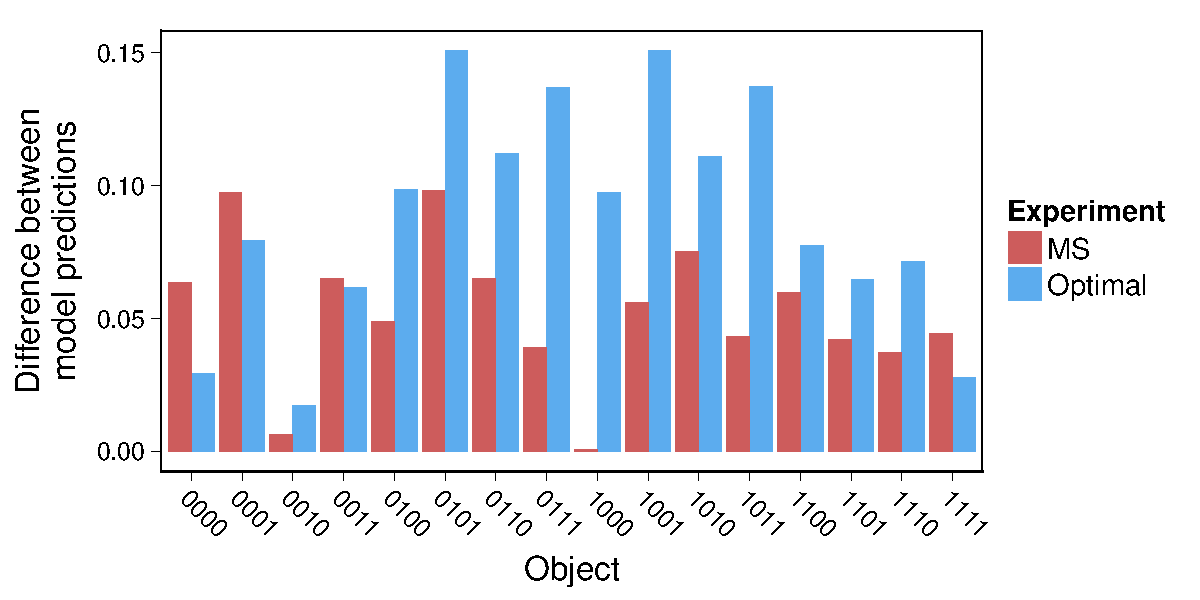
\includegraphics[width=0.9\columnwidth]{img/category-model-diffs.pdf}
  \caption{Difference between prototype and exemplar model predictions by object in the MS and optimal experiments. Optimal experiment has greater differences for most objects.}
  \label{fig:category-model-diffs}
\end{figure}


\begin{figure}[h]
(a) \\
\includegraphics[width=0.9\columnwidth]{img/category-eig-dist.pdf}\\
(b) \\
\includegraphics[width=0.9\columnwidth]{img/category-aig-curve.pdf}
\caption{(a) Distribution of EIG for all category learning experiments on a single participant. MS has low EIG. (b) AIG versus number of participants in analysis (error bars are 95\% bootstrapped confidence intervals). MS requires more participants to achieve maximum AIG.}
\label{fig:dist}
\end{figure}

\subsection{Empirical validation}

To validate our EIG calculations, we ran the MS and optimal experiment with 60 participants each.
Figure~\ref{fig:dist}b shows that the optimal experiment we found for a single participant is indeed better than the MS experiment ($n$=1, blue greater than red).
For $n$=1, the mean actual information gain (AIG) for the optimal experiment is 0.15, whereas it is 0.026 for the MS experiment.
This 5-fold difference is even greater than the 2.5-fold difference predicted by EIG.
In addition, by incrementally introducing more data, we observe that both experiments eventually reach maximal AIG but the optimal experiment takes only 10 participants to do so whereas the MS experiment takes around 30 participants.
Thus, the optimal experiment could provide the same amount of information for a third of the experimental cost.

% and illustrates how automated experiment design can outperform human intuition. In particular, this case study demonstrates the efficacy of OED in psychology for discrete and non-ordinal experiment spaces, large combinatoric experiment spaces, and parametric model classes.

\section{Related work}

The basic intuition behind OED---to find experiments that maximize some measure of expected informativeness---has been independently discovered in a number of fields, including physics \citep{vanDenBerg2003}, chemistry \citep{Huan2010}, biology \citep{Vanlier2012, Liepe2013}, psychology \citep{Myung2009}, and statistics \citep{Lindley1956}.%., and machine learning \citep{Golovin2010}.

Previous work, however, has either been too narrow for general use or required too much statistical and computational expertise.
For example, \cite{Liepe2013} devised a method for finding experiments that optimize information gain for parameters of biomolecular models (ODEs with Gaussian noise).
\cite{Myung2009} described a more general optimization method but this requires users to select their own utility function for the value of an experiment and implement inference on their own.
For example, they compared six memory retention models using Fisher Information Approximation as a utility function and performed inference using a custom annealed SMC algorithm.
Such ``bring-your-own'' requirements impose a significant burden on users and are a real barrier to entry.

By contrast, our OED system is general and practical, which allows users to rapidly explore different spaces of models, experiments, and inference algorithms.
This probabilistic programming based approach naturally handles certain challenging features of cognitive science experiments: human participants give noisy responses, experimental results are sensitive to the size of one's sample, and computational models often do not make direct predictions about experimental data, instead requiring \emph{linking functions} to convert model output into predictions about data.
Additionally, our work is the first to demonstrate that expected information gain is a reliable predictor of actual information gain.

\section{Conclusion}

Cognitive scientists aim to design experiments that yield informative results.
\texttt{webppl-oed} partially automates experiment design, searching for experiments that maximally update beliefs about the model distribution.
With our approach, scientists write their models as probabilistic programs, define a space of possible experiments and results, and hand these to OED for experiment selection.
We stress that the tool \emph{complements} scientists; it does not replace them.
Our tool merely eliminates the need to manually comb large spaces of potential experiments, which is time consuming, tedious, and prone to bias, such as a preference for local qualitative differences at the expense of ultimate quantitative information gain.
The real ingenuity---devising empirical paradigms and building models---must still come from the scientist.

Our approach suggests a number of interesting directions for future work.
First, OED can be computationally challenging---our software currently does not scale up to huge response or experiment spaces, so there is still room for optimizing search algorithms.
Second, we have examined model comparison problems where there are a finite number of models.
We believe that our approach also works in (1) parameter learning settings where the goal is to conduct experiments that best update beliefs about continuous parameters of a model, and (2) model comparison problems where a finite number of models each have continuous parameters that are unknown and must be integrated over.

%First, we chose KL divergence between posterior and prior as our informativeness measure because it is a well-known divergence function, but other choices (e.g., TV distance) might also be suitable.

Lastly, we have restricted attention to ``one-shot'' experiments, but it would be useful to extend our work to sequential settings such as adaptive testing.
Adaptive testing can be formulated as a problem of information gain of \emph{sequences} of experiments, which produce dependent and non-iid responses.
Some preliminary work suggests that \texttt{webppl-oed} can be profitably extended to the adaptive setting.


%
%Fourth, we have ignored the cost of experiments, but it would be worth explicitly taking this into account.
%Our informativeness approach could be usefully integrated with for real-world applications (e.g., MRI studies of rare patient populations, expensive aerospace experiments).

% \bibliographystyle{ieeetr}
\bibliographystyle{apacite}
\bibliography{oed_cogsci_2018}

\end{document}
